
\section{Analysis strategy}
\label{sec:analysis}


In section we describe our analysis strategy, and in particular
the classification of each individual event into
different categories according to the event topology.

First of all we discuss the settings and nomenclature that
we will use for jet clustering in this work.
%
Then we move to discuss how $b$-tagging is simulated,
following closely the ATLAS techniques.
%
Then we discuss the categorisation of events between different
topologies, and how we can prioritise among them.


\subsection{Jet reconstruction}

In our analysis we will use different types of jet definitions,
depending of the type of analysis that needs to be performed.
%
Therefore, we being by enumerating the choices that we make.
%
The starting point after the parton shower is the clustering
of all final state particles.
%
In this work all the jet reconstruction algorithms
are obtained from the {\tt FastJet} program~\cite{Cacciari:2011ma},
v3.1.0.
%
We adopt the following terminology for the different types of jets
that we will use in this work:

\begin{itemize}
\item {\it Small-$R$ jets}.

  These are jets  reconstructed with the
  anti-$k_T$ clustering algorithm~\cite{Cacciari:2008gp} with $R=0.4$ radius.
  %
  When reconstructing small-$R$ jets, we will keep only
  those with transverse momentum $p_T \ge 40$~GeV
  and pseudo-rapidity $|\eta|<2.5$ within the central
  acceptance of ATLAS and CMS, jets that fail to satisfy these
  conditions are discarded

  They are required to have $p_T > 50$~GeV and $|\eta|<2.5$.

\item {\it Large-$R$ jets}.

  These jets are also constructed with the
  anti-$k_T$ clustering algorithm, now using a $R=1.0$ radius.
  %
  In order to be accepted, these large-$R$ jets should
  satisfy  $p_T \ge 200$~GeV and lie in a pseudo-rapidity range by
  $|\eta|<2.0$.
  %
  If these conditions are not satisfied, the jet is discarded.
  %
  The more restrictive range  in pseudo-rapidity
  as compared to the small-$R$ jets,
  is motivated by mimicking the  experimental requirements
  in ATLAS and CMS
  related to the track-jet-based calibration.

  In addition to the basic $p_T$ and $\eta$
  selection requirements, large-$R$ jets should also
  satisfy the  BDRS mass-drop tagger~\cite{Butterworth:2008iy}
  conditions, in order
  to enhance the discrimination of the signal over the background
  events.
  %
  For the BDRS mass-drop tagger, we use the {\tt FastJet} default
  parameters of  $\mu = 0.67$ and $y_{\textrm{cut}}= 0.09$.
  %
  Before the mass-drop tagger is applied, the large-$R$ jet
  constituents are reclustered with the Cambridge/Aachen
  algorithm.


  
\item {\it Small-$R$ subjets}.

  Once we have reconstructed a suitable large-$R$ jet, important
  information can be obtained by looking at the kinematics of
  the small-$R$ subjets.
  %
  These subjets will be obtained by reclustering the constituents
  of the large-$R$ jet, always with the  anti-$k_T$ algorithm,
  but this time with a smaller radius parameter $R=0.3$.
  %
  As we will discuss below, these small-$R$ subjets are the key of
  the $b$-tagging in the boosted category.
%
  \end{itemize}


\subsection{$b$-tagging}

Given the final state that needs to be reconstructed, the
optimisation of the $b$-tagging capabilities of the
LHC experiments is an essential requirement.
%
The $b$-tagging used in this feasibility study is inspired
in the current and projected ATLAS settings, and below
we also comment on the differences and similarities with the
corresponding CMS strategy.
%
For each type of jet defined above, a different
$b$-tagging strategy is used, as we discuss now.

\begin{itemize}

\item {\it Small-$R$ jets}.

  These are $b$-tagged as follows.
  %
  If a small-$R$ jet has at least one $b$-quark among their constituents,
  it will be tagged as a $b$-jet with probability $f_b$.
  %
  If no $b$-quarks are found among the constituents
  of this jet, it can be still be tagged as a $b$-jet with
  a mistag rate of $f_l$.
  %
  Note that the probability of tagging a jet is not increased
  if more than one $b$-quark is found among the jet constituents.

  \item {\it Large-$R$ jets}.

    Large-$R$ jets are $b$-tagged by ghost-associating anti-$k_T$ $R=0.3$
    subjets (defined as above) to the original large-$R$ jets.
    %
    In particular,
    a large-$R$ jet is considered  double-$b$-tagged if both
    the leading and subleading subjets (where the ordering
    is done in the subjet $p_T$) are both individually $b$-tagged.
    %
    Note that we only attempt to $b$-tag the two leading subjets:
    trying to $b$-tag all subjets above the $p_T$ cut degrades
    the signal significance due to the increase in combinatorics.

    Therefore, in this work we will exploit the capabilities of
    the LHC experiment of double-$b$-tagging inside large-$R$ jets.
    %
    Below we comment on the dependence of our results if single-$b$-tagging
    would be performed also for the large-$R$ jets, as done
    for the small-$R$ jets.

    Concerning the $b$-tagging probabilities and the
    light jet mistag probabilities, there are taken
    the same as for small-$R$ jets.
    %
    Therefore, a large-$R$ jet where the two leading
    subjets have at least one $b$-quark will be tagged
    with probability $f_b^2$, if only one of the two leading
    subjets has a $b$-quark then the tagging probability is
    $2f_bf_l$, and if none of the two have $b$-quarks
    as constituents, the mistag rate will be
    $f_l^2$.


\end{itemize}

Concerning the actual values of the $b$-tag probability $f_b$ and
the $b$-mistag probability of light jets $f_l$, in this work
we adopt as baseline the values $f_b=0.8$ and $f_l=0.01$.
%
In Sect.~\ref{sec:optimisation} we study the dependence of
our results against variations of $f_b$ and $f_l$ both
using more conservative and more aggressive values.
%
There we also study the dependence of the results
on other analysis settings related to the performance of
the experiments, for example by varying the momentum smearing.

\subsection{Event categorisation and cut flow}

After having introduced the types of jet reconstruction
that we will use, as well as the $b$-tagging strategy,
we need to discuss the analysis strategy, including
the event categorization and the cut flow.

The basic idea of this work is the same as in Ref.~\cite{Gouzevitch:2013qca}:
rather than selecting only a specific event topology, such as boosted
or resolved, we aim to consistently combine the information from
the three possible event topologies: boosted, intermediate and
resolved, which we define now.
%
An important difference as compared to~\cite{Gouzevitch:2013qca}
is that here each category is optimised separately, and then
a exclusive categorisation is defined starting from the topology
where the signal significance is the largest.


Let us therefore define the three event categories that
we use in this work:
\begin{itemize}
\item {\it Boosted category}.

  A given event is assigned to the boosted category if it
  contains at least two large-$R$ jets, defined as above,
  and of the tow leading large-$R$ jets have been double-$b$-tagged.
  %
 Therefore, each of these two large-$R$ $b$-tagged jets correspond to the
 decay products of one Higgs boson candidate.

\item {\it Intermediate category}.

  An event is assigned to the intermediate category if
  at least one large $R$ $b$-tagged jet is present.
  %
  If more than one is found, then the leading large-$R$ jet
  is assigned to be the first Higgs candidate.
  %
  In addition, we require at least two small-$R$ jets,
  which must be separated with respect to the large-$R$
  jet by at least an angular separation of $\Delta R\ge 1.0$.
  %
  The small-$R$ jets must be $b$-tagged as well.
  %
  Then, the second Higgs boson candidate is reconstructed
  by selecting the two small-$R$ jets that minimize the difference
  between the invariant mass of the large-$R$ jet, $m_{lR}$,
  with the invariant mass of the sum of the two small-$R$ jets,
  $m_{sR_1+sR_2}$, that is, ${\rm min}\lp m_{lR} -
  m_{sR_1+sR_2}\rp$.

\item {\it Resolved category}.

  Finally, let us define the resolved category.
  %
  An event is assigned to this category
  if at least
  four $b$-tagged small-$R$ jets are present.
  %
  The two Higgs candidates are then reconstructed out of the
  leading four small-$R$ jets in the event
  by considering all possibilities of forming two pairs of jets
  with invariant masses $m_{sR_1+sR_2}$ and 
$m_{sR_3+sR_4}$, respectively, and choosing the configuration that minimizes their difference $|m_{sR_1+sR_2} - m_{sR_3+sR_4}|$. 
  %
  The requirement of restricting this selection to only the four
  leading small-$R$ jets arises from the need to reducing the
  combinatorics from the fakes.
\end{itemize}

In addition, events from each category need to satisfy the usual
Higgs mass window cut, defined by
the following condition
\be
|m_{h,j} - 125| < 40~{\rm GeV} \, , j=1,2 \, ,
\ee
where $m_{h,j}$ is the invariant mass of the two Higgs candidates
reconstructed as explained above.
%
We note that this cut is substantially looser as the corresponding
cut used in the ATLAS and CMS $h\to b\bar{b}$ analysis: the motivation
for this is that the MVA will take care of the optimisation of each cut.



In Table~\ref{sec:categorisation} we summarize the definitions of each
category.
%
We emphasize that each category is not exclusive of the others,
and in general there can be a substantial overlap
between the different categories.




%%%%%%%%%%%%%%%%%%%%%%%%%%%%%%%%%%%
\begin{table}[h]
  \centering
  \small
  \begin{tabular}{c|c|c|c}
    \hline
    &  Boosted  &  Intermediate  &  Resolved  \\
    \hline
    \hline 
    Jet selection  &  $\ge 2$ large-$R$ jets  & 1 large-$R$ jet, $\ge 2$ small-$R$
    jets  &  $\ge$ 4 small-$R$ jets \\
    \hline
    Jet cuts  & $p_T \ge 200$ GeV   &  $p_T \ge 200$ GeV (large-$R$ jet)
    &  $p_T \ge 40$ GeV \\
    &  & $p_T \ge 40$ GeV (small-$R$ jets)   &    \\
    &   $|\eta|<2.0$  & $|\eta|<2.0$ (large-$R$ jet) & $|\eta|<2.5$ \\
    &        & $|\eta|<2.5$ (small-$R$ jet)  &  \\
    \hline
    $b$-tagging  & 2 double-$b$-tags  & 1 double-$b$-tag & 4 single-$b$-tags \\
      &  & and 2 single-$b$-tags  &  \\
    \hline
    \end{tabular}
  \caption{\small Definition of the three event categories used in this
    work, together with the corresponding basic kinematical cuts.
\label{sec:categorisation}
  }
\end{table}
%%%%%%%%%%%%%%%%%%%%%%%%%%%%%%%%%%%%%%


We now justify some of the cuts that we are using.
%
As mentioned before, the cuts in each category are separately
optimised in an inclusive analysis: it is only we have determined
which is the dominant category that the analysis is made exclusive.
%
We begin with the boosted category.
%
In Fig.~\ref{fig:cutplots1} we show
the $p_T$ distribution of the
  leading large-$R$ jet in the boosted category, comparing
  the shapes of the distribution in signal and background events.
  %
  All distributions have been normalized to their total integral.


%%%%%%%%%%%%%%%%%%%%%%%%%%%%
\begin{figure}[t]
\begin{center}
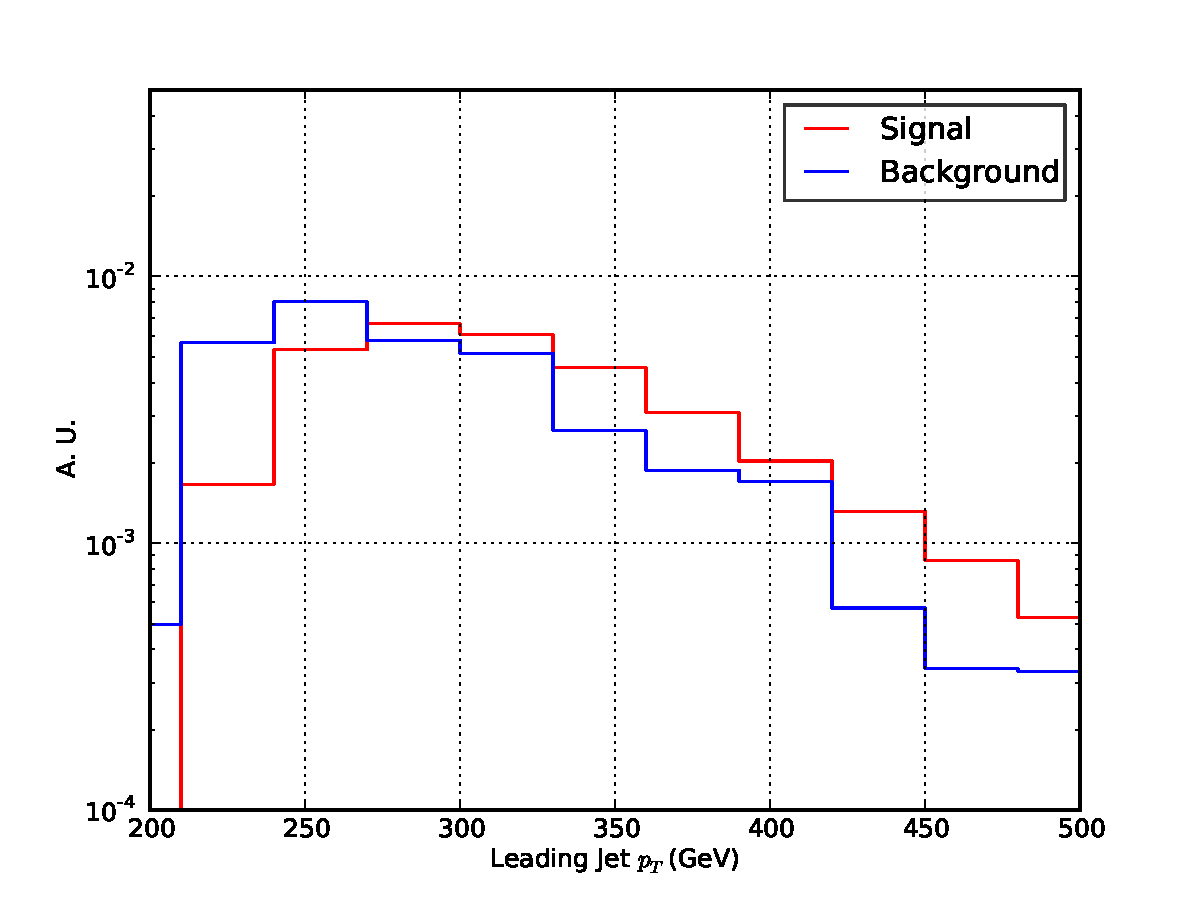
\includegraphics[width=0.48\textwidth]{plots/pt_H0_res_C1_boost.pdf}
\caption{\small Left plot: the $p_T$ distribution of the
  leading large-$R$ jet in the boosted category, comparing
  the shapes of the distribution in signal and background events.
  %
  All distributions have been normalized to their total integral.
}
\label{fig:cutplots1}
\end{center}
\end{figure}
%%%%%%%%%%%%%%%%%%%%%%%
